\chapter{Metodologia}
Um dos objetivos deste estudo é estabelecer uma metodologia para comparar os distúrbios de gravidade de um ponto ou conjunto de pontos, a partir de um MGG. Dessa forma, definimos uma estratégia na qual alguns elementos do campo de gravidade predito pelo modelo de harmônicos esféricos são comparados com os mesmos elementos observados \textit{in situ}. Por conseguinte, é possível analisar a viabilidade desta metodologia em relação à acurácia das estimativas. Para esta avaliação foram utilizados conjuntos de dados de gravimetria e altimetria.

\section{Área de estudo}

A área onde o levantamento terrestre foi realizado corta longitudinalmente a Bacia do Parnaíba (Figura \ref{fig:bacia do parnaiba}). Este estudo produzido pela equipe de geofísica do \textit{Observatório Nacional} (ON) em parceria com a \textit{British Petroleum} (BP) serviu de base para o desenvolvimento deste trabalho, possibilitando confrontar dados terrestres com os dados obtidos via MGG.

\begin{figure}[h]
	\centering
	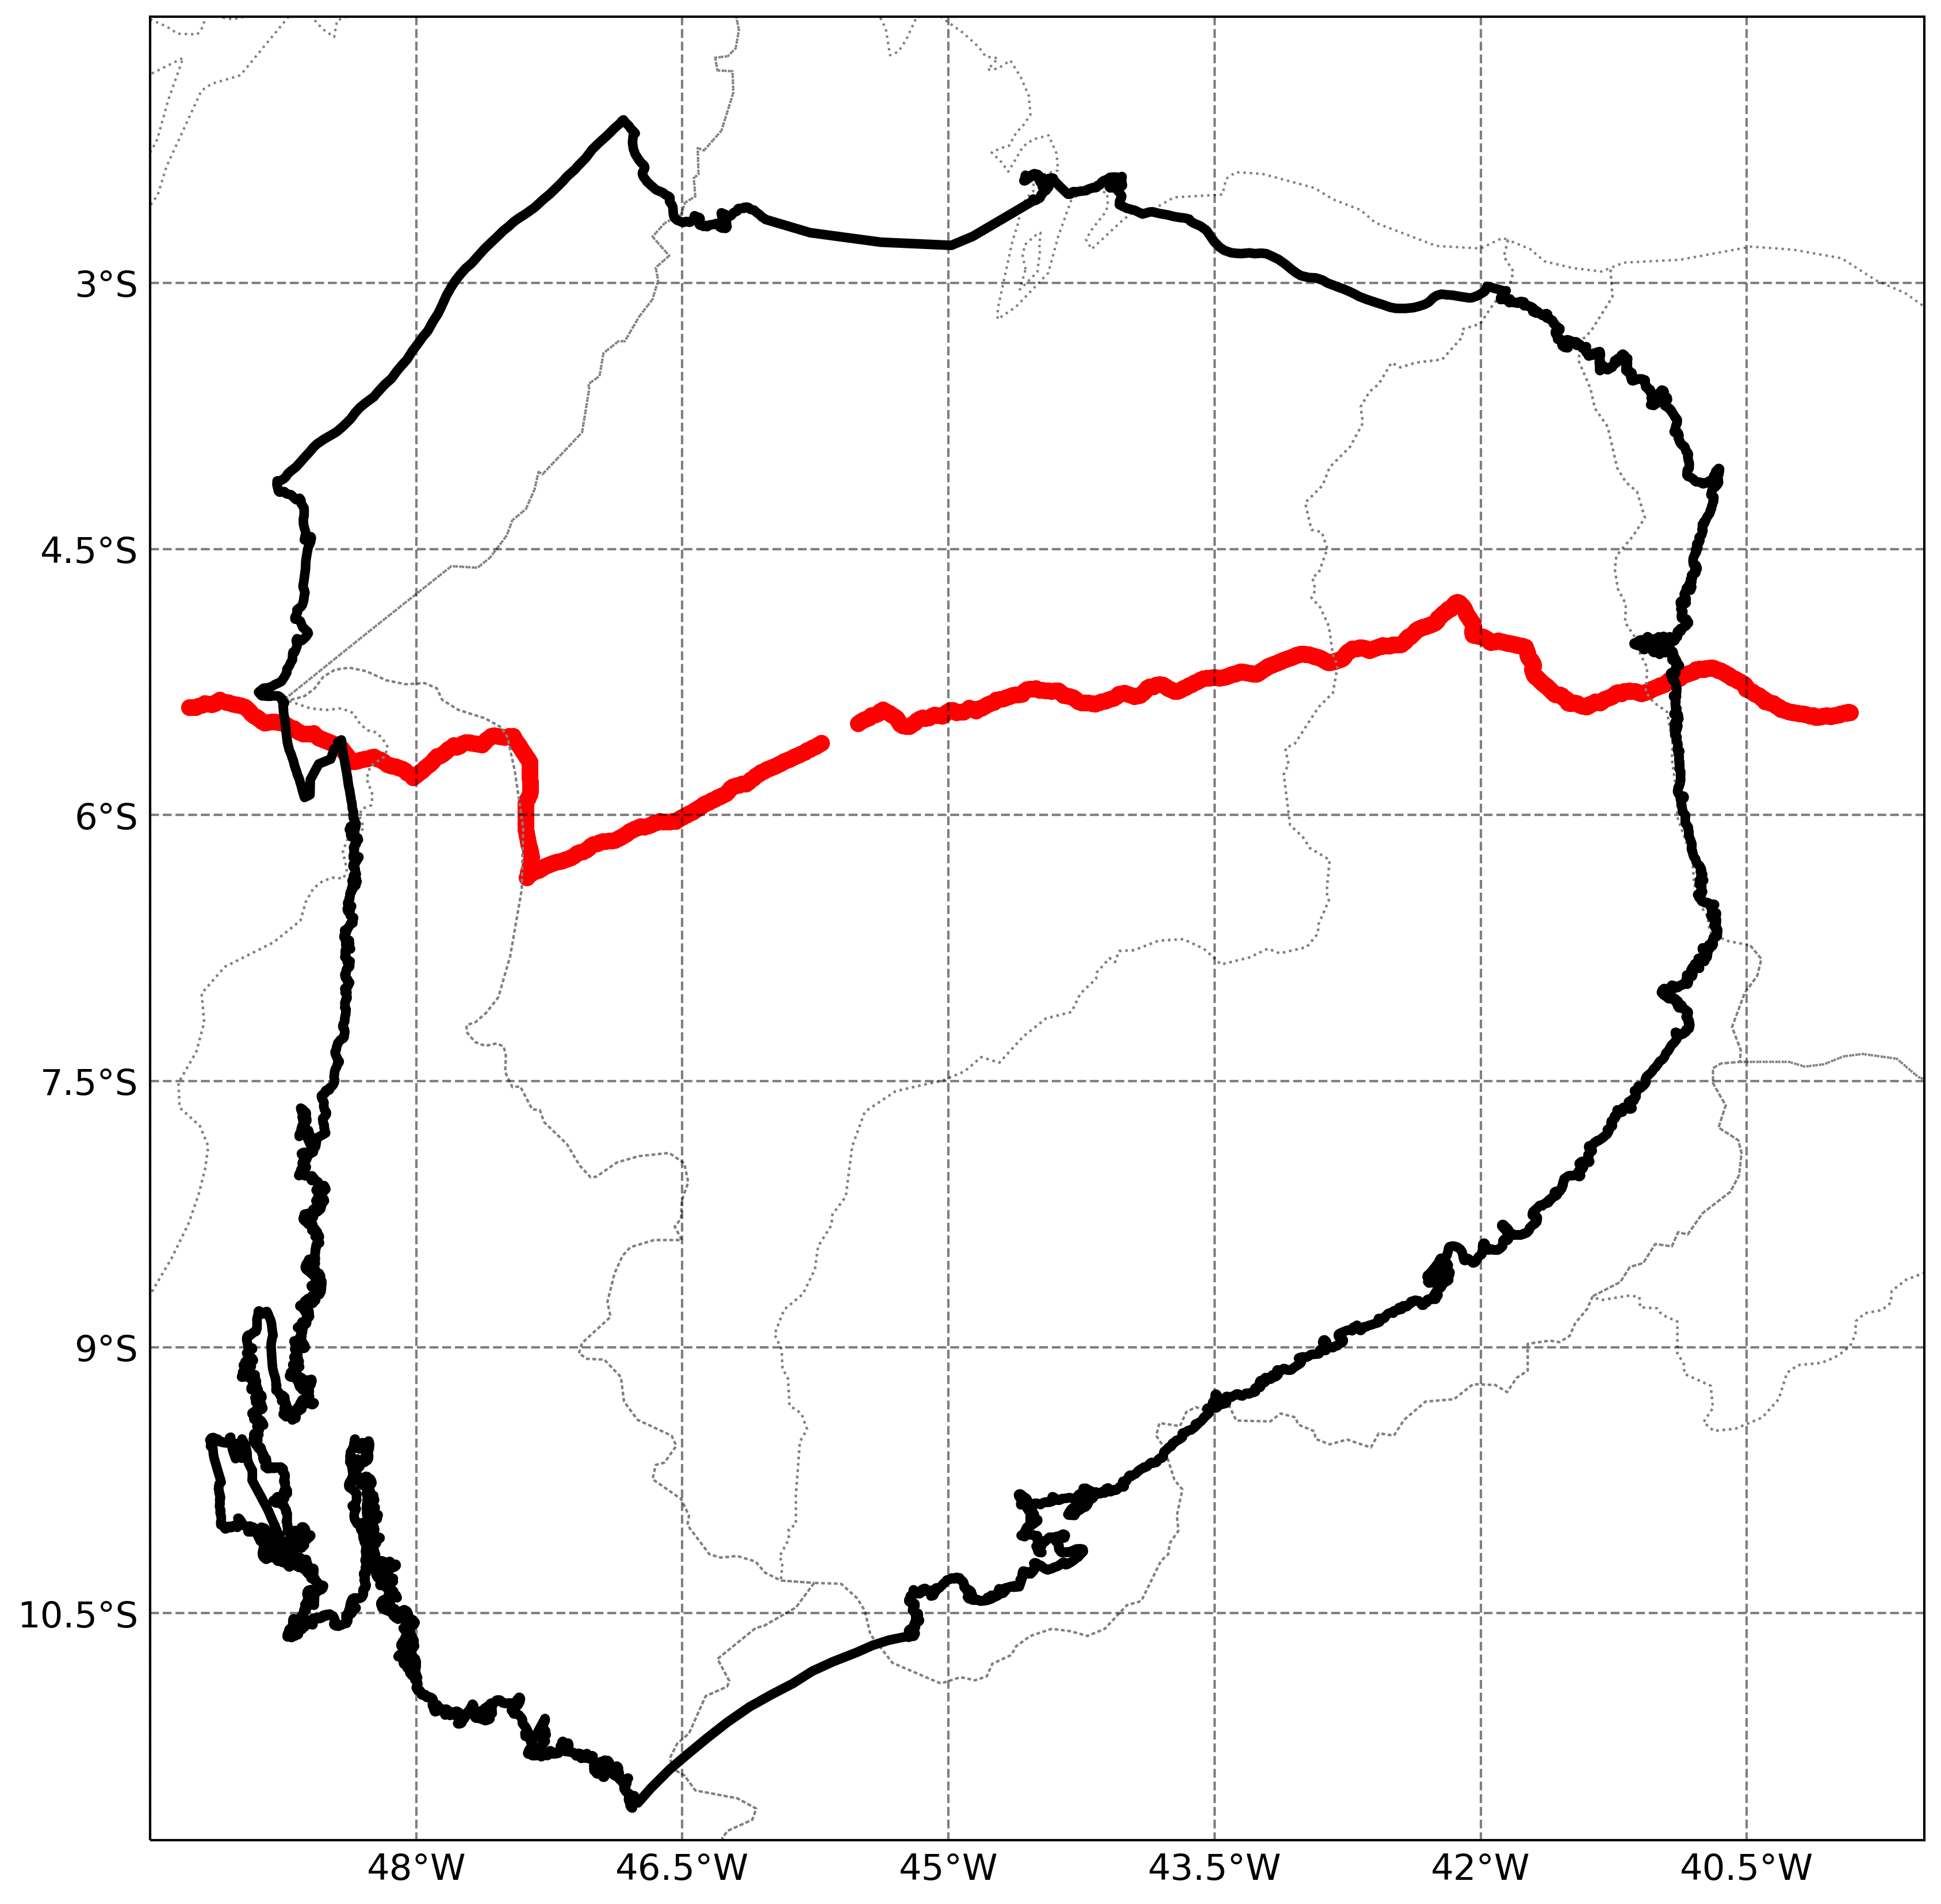
\includegraphics[scale=0.25]{figs/bacia do parnaiba.png}
	\caption{Mapa da região da Bacia do Parnaíba, em vermelho o perfil das estações onde foram adquiridos os dados terrestres.}
	\label{fig:bacia do parnaiba}
\end{figure}

A bacia do Parnaíba está localizada na região nordeste brasileira, na sua porção ocidental e em partes de áreas vizinhas, distribuindo-se pelos estados do Ceará, Bahia, Piauí, Maranhão, Tocantins e Pará, abrangendo uma área de cerca de $660.000km^{2}$ \cite{article_parnaiba}. É classificada como uma bacia intracratônica, um tipo  comumente localizado em crosta continental estável e espessa, mas relativamente fina se comparada à sua extensão e geralmente com formação associada à separação de supercontinentes em processos de subsidência termal ao longo de sua formação \cite{vaz2007_parnaiba}. Comumente, bacias sedimentares com este histórico são divididas em várias megassequências que podem ter sido formadas em diferentes épocas sob regimes tectônicos distintos. Logo, é necessária uma análise cuidadosa das diferentes fases de formação da bacia \cite{bacias_intracratonicas}. Ainda assim, a morfologia destas bacias está associada, em geral, a um mecanismo tectônico primário, restringindo os mecanismos secundários a modificações menores \cite{allen2012cratonic}. A Bacia do Parnaíba desenvolveu-se sobre embasamento continental durante a estabilização da Plataforma Sul-Americana, e, por correlação com rochas existentes nas faixas de dobramentos, maciços medianos e outras entidades complexas situadas nas bordas ou proximidades da bacia, deduz-se que o seu substrato é formado de rochas metamórficas, ígneas e sedimentares, cujas idades abrangem um intervalo do Arqueano ao Ordoviciano \cite{tese_bacia_parnaiba}. A estrutura geológica define a topografia da região com regiões planas entre os vales, com altitudes de  $\approx 800$m, sendo as cotas maiores localizadas preferencialmente na borda leste onde se localiza uma feição de Serra. 

\section{Descrição dos dados}

\subsection{Gravimetria terrestre}

O levantamento de campo realizado pela equipe de Geofísica do ON percorreu aproximadamente 1200km, iniciando na margem leste da bacia, no estado do Ceará e finalizando na margem oeste, no estado do Pará. O perfil traçado em vermelho no mapa da Figura \ref{fig:bacia do parnaiba} corresponde ao caminho feito durante o levantamento, cujo objetivo original era realizar um levantamento gravimétrico terrestre cortando a bacia do Parnaíba de leste a oeste.

O gravímetro diferencial Autograv-CG5 da Scintrex (Figura \ref{subfig:gravimetro-gps}.a) e o receptor GNSS da Trimble (Figura \ref{subfig:gravimetro-gps}.b), foram os equipamentos utilizados para medir a gravidade e as coordenadas plani-altimétricas ao longo de todo o levantamento, respectivamente. O gravímetro diferencial é um equipamento bastante comum em levantamentos de campo devido a suas características técnicas e simplicidade de operação \cite{cg5} e com precisão da ordem de 1$\mu$Gal \cite{on_cg5}. Por si só, ele não é capaz de medir a gravidade absoluta, já que a sua leitura consiste em medir a diferença entre estações adjacentes. Consequentemente, a conexão das estações do perfil com pelo menos uma estação de uma rede gravimétrica conhecida, se faz obrigatória. Apesar do equipamento possuir uma antena de GPS própria, esta é somente usada para sincronizar o relógio interno com a hora precisa da constelação de satélites. Isso permite ao gravímetro realizar algumas reduções gravimétricas de forma automática, como as reduções de deriva instrumental (i.e., devido ao desgaste do equipamento) e de maré (i.e., fruto da interferência luni-solar) \cite{geodesia}. É também possível configurar o gravímetro para aplicar reduções de terreno ao dado, porém esse não fora aplicado. O GPS do gravímetro não contém a precisão necessária para determinar as coordenadas planimétricas e também não é capaz de mensurar a altitude geométrica do ponto. Dessa forma, o receptor diferencial da Trimble, cujas coordenadas plani-altimétricas são observadas com precisão centimétrica \cite{trimble,gps}, foi o utilizado nesta expedição. Neste caso, um receptor chamado base é fincado em um local confiável e remoto, livre de interferências, normalmente afastado das estações gravimétricas que caracterizam o levantamento, para ter comunicação direta com a constelação de satélites. Um outro receptor denominado móvel realiza as medidas das coordenadas plani-altimétricas das estações gravimétricas do levantamento. O tempo de exposição e comunicação entre os receptores são essenciais para a obtenção das coordenadas com alta precisão. A tabela \ref{tab:dados_terrestre} resume brevemente a gravimetria e altimetria observadas em campo.

\begin{table}[h]
	\centering
	\caption{Resumo dos dados observados.} \label{tab:dados_terrestre}
	\begin{tabular}{c|c|c|c|c}
		
		Dados & Mínimo & Máximo  \\ 
		\hline                               % para uma linha horizontal
		Latitude (º) & 4,8ºS & 6,35ºS \\
		Longitude (º) & 39,91ºW & 49,28ºW \\
		Gravidade absoluta (mGal) & 977893.4 & 978048.18 \\
		Altitude geométrica (m) & 74,54 & 718,83
		% não é preciso quebrar a última linha	
	\end{tabular}
\end{table}

\begin{figure}[!ht]
	\centering
	\subfloat[Gravímetro relativo \textit{Autograv CG-5} da \textit{Scintrex Ltda.}.]{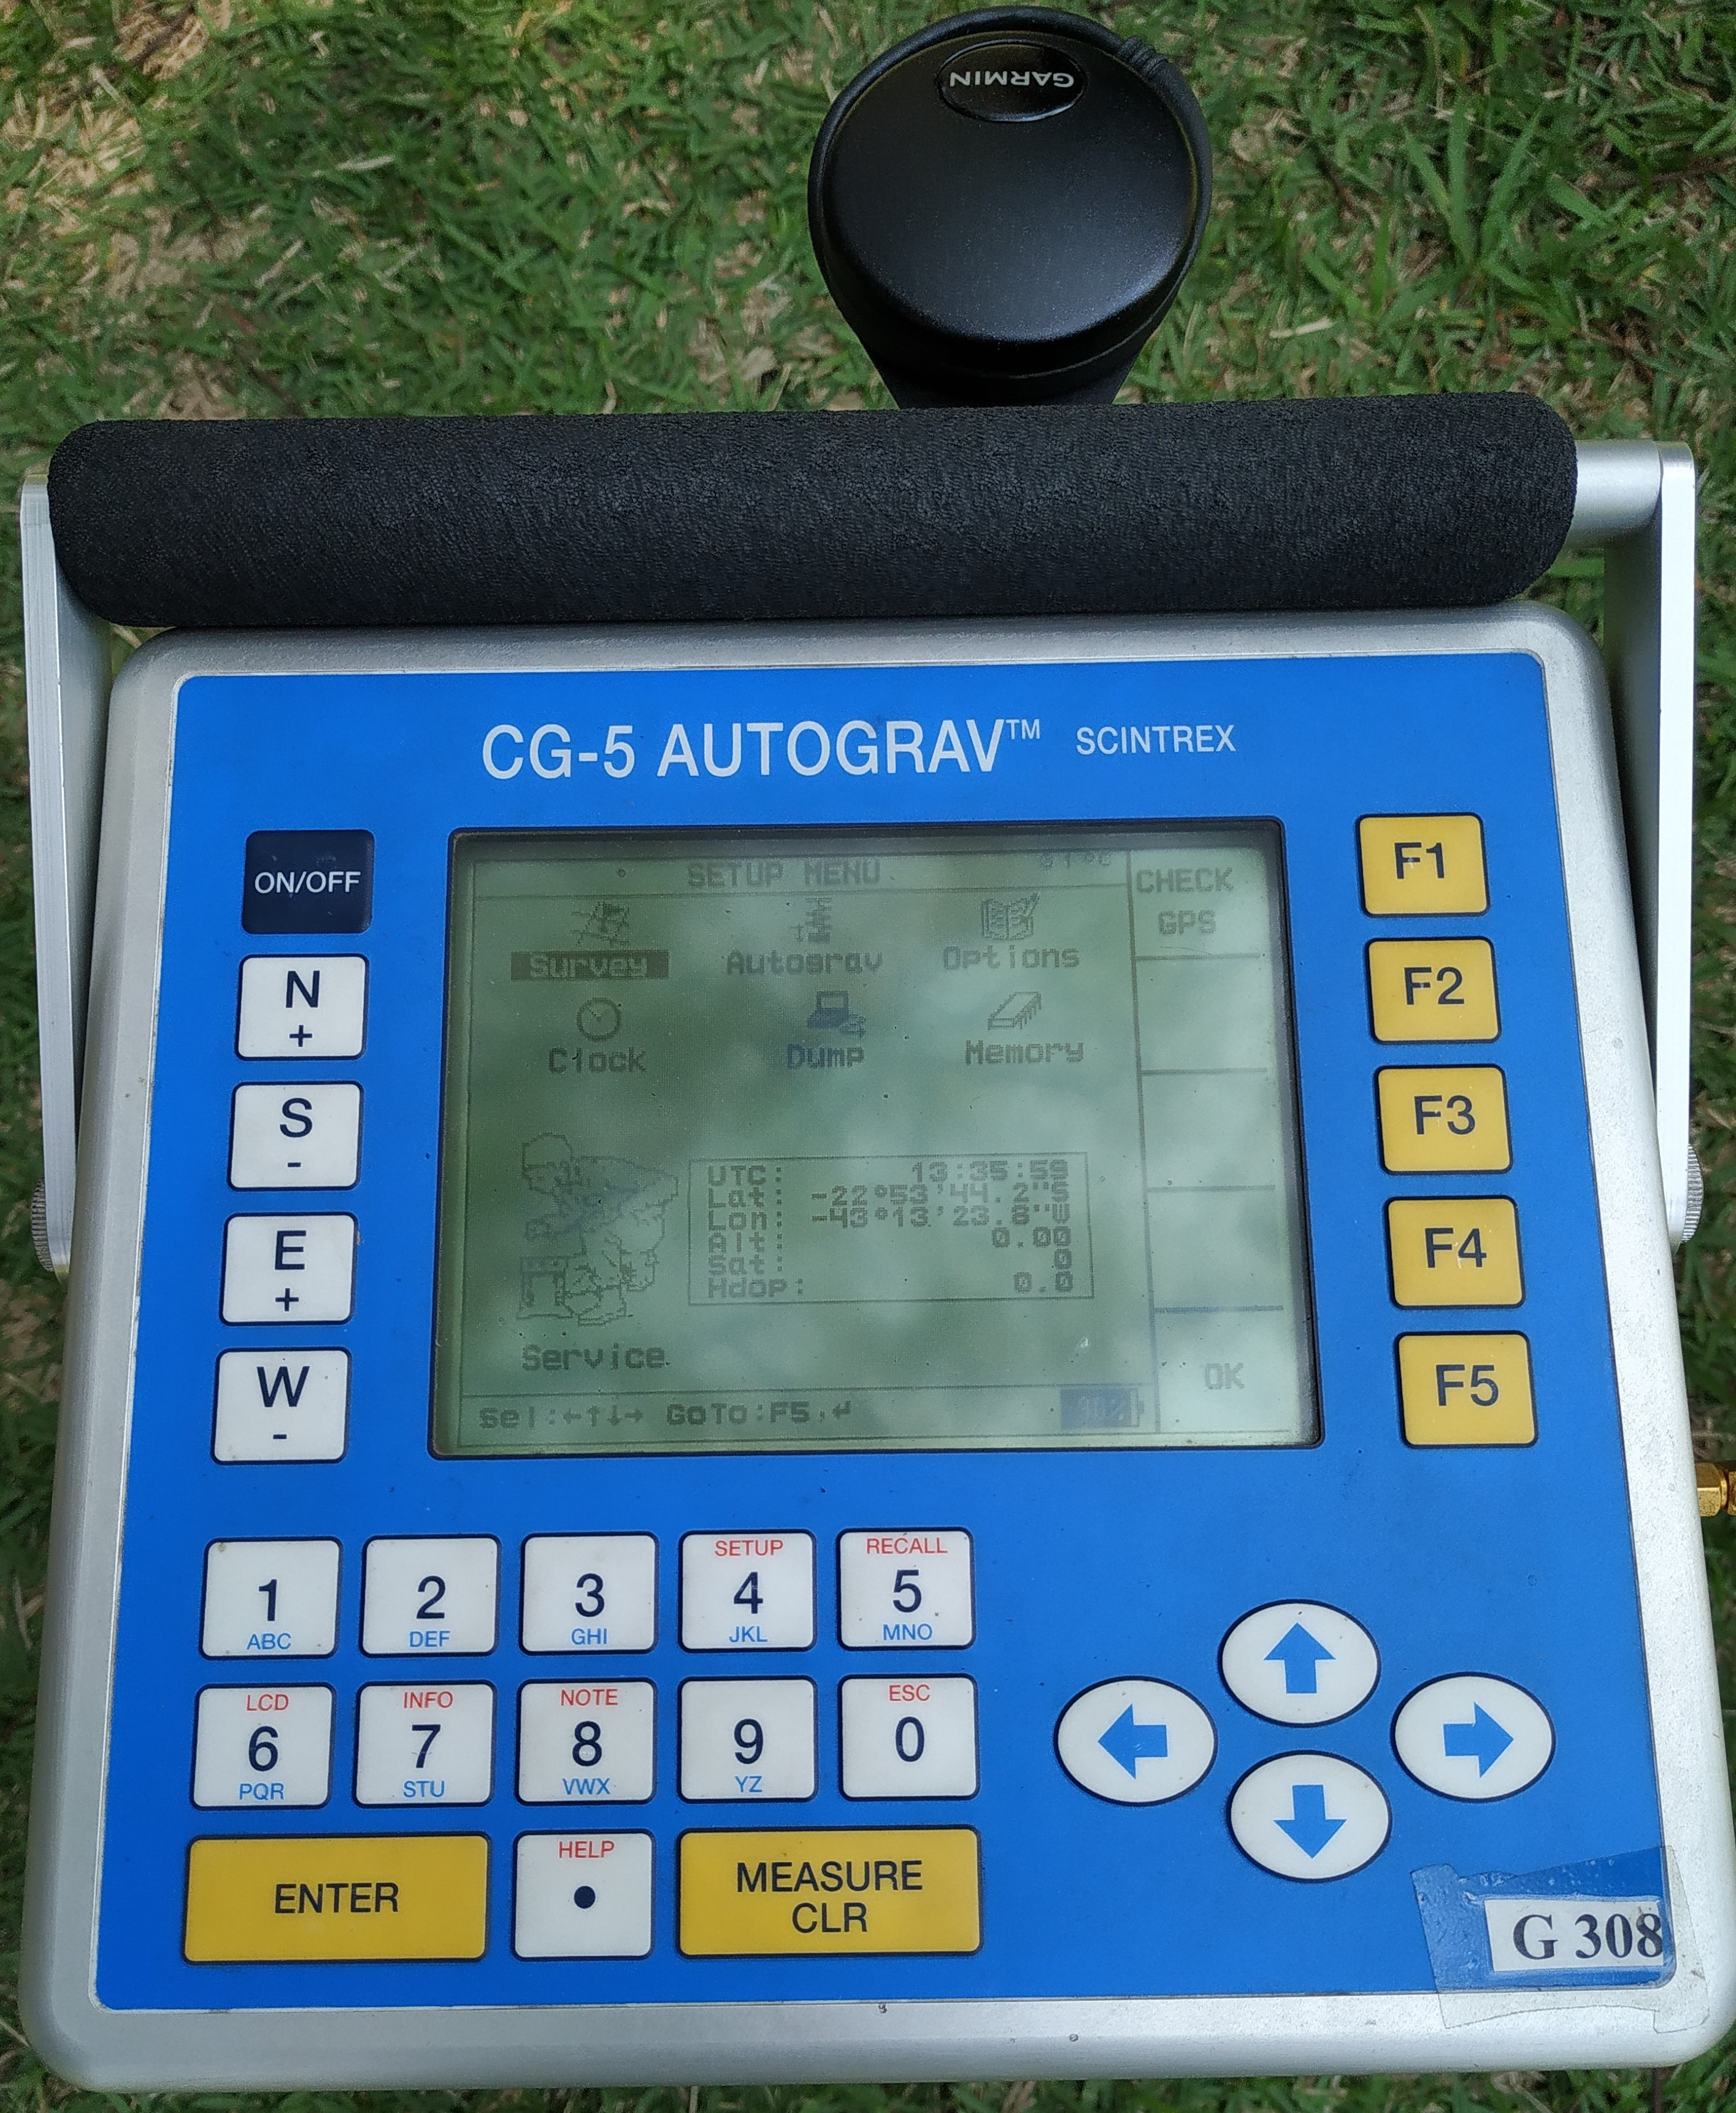
\includegraphics[width=5cm,height=5cm]{figs/cg5.jpg}}
	\qquad
	\subfloat[Aquisição terrestre com o \textit{Autograv-CG5 } junto ao \textit{GPS Trimble} utilizado para mensurar as coordenadas plani-altimétricas. Retirado de: \textit{Topocart}.]{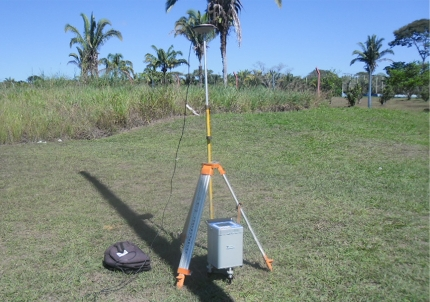
\includegraphics[width=5cm,height=5cm]{figs/2b}}
	\caption{Equipamentos necessários para realizar um levantamento gravimétrico terrestre.}  
	\label{subfig:gravimetro-gps}
\end{figure}

\subsection{Gravimetria por satélite}

O conjunto de dados de satélite é de domínio público e está disponibilizado no site do ICGEM. Dentro do banco de dados do $ICGEM$, há uma série de modelos que calculam elementos da gravidade. Dentre eles, foi utilizado o modelo \textit{EIGEN-6C4}. Este foi escolhido por se tratar do modelo de gravidade global que possui expansão em harmônicos esféricos de maior grau e ordem, iguais a 2190 \cite{eigen}, em comparação com outros existentes. Trata-se do maior truncamento proposto e que, portanto, melhor representa os sinais de alta frequência contidas nos dados de gravidade.Deste modelo, foram utilizados os funcionais \textit{gravity\_earth} e \textit{gravity} associados às malhas regulares e estações terrestres, respectivamente, compondo o conjunto de dados preditos.
\subparagraph{Funcional \textit{gravity$\_$earth}:} De acordo com \citeonline{barthelmes2009}, o funcional \textit{gravity\_earth}, selecionado pela aba \textit{Regular grids}, aplica a técnica de expansão em harmônicos esféricos ao potencial de gravidade, para calcular a gravidade absoluta sobre a $SFT$, sendo esta a magnitude do gradiente de $W$ (equação \ref{eq:vetor_gravidade_g}) nas respectivas coordenadas planimétricas escolhidas pelo usuário. Para mais detalhes acerca dessa aplicação, o leitor é convidado à \citeonline{barthelmes2009}. As malhas regulares de satélite abrangem uma área definida pelas latitudes $0.2$º$S$ $\leq \varphi \leq$ $11.78$º$S$ e longitudes $39.5$º$W$ $\leq \lambda \leq$ $50$º$W$, ambas em graus decimais e com espaçamento de $0.03$º. A escolha dos limites $\varphi$ e $\lambda$ está relacionada com a localização da Bacia do Parnaíba, que consta como o alvo do estudo. Estas malhas serviram para analisar a bacia sob uma ótica regional. O espaçamento possibilitou uma amostragem maior, com $135837$ pontos analisados. Este funcional gera um arquivo com as seguintes colunas: longitude e latitude em graus decimais; as altitudes ortométricas em metros de cada ponto definido pelo usuário; a gravidade absoluta em mGal. A tabela \ref*{tab:dados_sat} resume brevemente o conjunto de dados calculados pelo funcional \textit{gravity\_earth}. A variação entre o maior e o menor valor da gravidade absoluta obtida foi de $373$ $mGal$, enquanto as altitudes ortométricas tiveram uma variação de $1322.92$m. 

\begin{table}[h]
	\centering
	\caption{Resumo dos dados calculados pelo funcional \textit{gravity\_earth}.} 
	\label{tab:dados_sat}
	\begin{tabular}{c|c|c|c|c}
		
		Dados & Mínimo & Máximo  \\ % Note a separação de col. e a quebra de linhas
		\hline                               % para uma linha horizontal
		Latitude (º) & 0,2ºS & 11,78ºS \\
		Longitude (º) & 39,5ºW & 50ºW \\
		Gravidade absoluta (mGal) & 977811.88 & 978184.24 \\
		Altitude ortométrica (m) & 0 & 1322.92
		% não é preciso quebrar a última linha	
	\end{tabular}
\end{table}
\subparagraph{Funcional \textit{gravity}:} O funcional \textit{gravity}, selecionado na aba \textit{User-defined points}, calcula, por meio da expansão em harmônicos esféricos, a gravidade absoluta como sendo a magnitude do vetor gravidade, ou seja, o módulo do gradiente de $W$, para quaisquer conjuntos de pontos de observação $(h, \varphi,\lambda)$ definidos pelo usuário \cite{barthelmes2009}. Para o cálculo através deste funcional, foram inseridas as coordenadas plani-altimétricas referentes às estações do levantamento terrestre, sobre as quais foram calculadas os respectivos valores de gravidade absoluta. Este funcional gera um arquivo com as seguintes colunas: longitude e latitude em graus decimais; as altitudes geométricas em metros de cada ponto definido pelo usuário; a gravidade em $mGal$ calculada sobre as coordenadas correspondentes. A tabela \ref{tab:dados_sat_pred} mostra as informações pertinentes a estes dados. Observa-se uma variação de $152$ $mGal$ entre os valores máximo e mínimo de gravidade absoluta e de aproximadamente $644$m nas altitudes geométricas observadas. 

\begin{table}[H]
	\centering
	\caption{Resumo dos dados calculados pelo funcional \textit{gravity}.}
	\label{tab:dados_sat_pred}
	\begin{tabular}{c|c|c|c|c}
		
		Dados & Mínimo & Máximo  \\ % Note a separação de col. e a quebra de linhas
		\hline                               % para uma linha horizontal
		Latitude (º) & 4,8ºS & 6,35ºS \\
		Longitude (º) & 39,91ºW & 49,28ºW \\
		Gravidade absoluta (mGal) & 977877.06 & 978029.54 \\
		Altitude geométrica (m) & 74,54 & 718,83 
		% não é preciso quebrar a última linha	
	\end{tabular}
\end{table}

\subsection{Altimetria por satélite}
O conjunto de dados disponibilizados na plataforma do $ICGEM$ não se restringem exclusivamente a elementos da gravidade. Dentre os funcionais disponíveis, também é possível calcular a topografia para qualquer região do globo. Portanto, foi adicionada ao estudo uma análise para comparar as altitudes  geométricas calculadas pelo modelo com as altitudes geométricas observadas. 
\subparagraph{Funcional \textit{h\_topo\_over\_ell}:} Este funcional é selecionado, assim como o \textit{gravity}, na aba \textit{User-defined points}. Ele calcula a altura da topografia sobre o elipsoide (i.e., a distância entre um ponto na $SFT$ e o elipsoide de referência), para um ponto ou conjunto de pontos informados pelo usuário. Este cálculo é feito por interpolação bilinear entre o modelo de elevação, relacionado ao geoide, somado a $N$. Este funcional gera um arquivo com as seguintes colunas: longitude e latitude em graus decimais; as altitudes geométricas em metros, calculadas através dos harmônicos esféricos. A tabela \ref{tab:dados_h_pred} mostra as informações pertinentes a estes dados. É importante ressaltar que as altitudes preditas por este funcional não foram utilizadas para o cálculo dos distúrbios de gravidade, detalhados na seção \ref{subsec:delta}, onde foram utilizadas as altitudes observadas. 

\begin{table}[H]
	\centering
	\caption{Resumo dos dados calculados pelo funcional \textit{h\_topo\_over\_ell}.}
	\label{tab:dados_h_pred}
	\begin{tabular}{c|c|c}
		
		Dados & Mínimo & Máximo  \\ % Note a separação de col. e a quebra de linhas
		\hline                               % para uma linha horizontal
		Latitude (º) & 4,8ºS & 6,35ºS \\
		Longitude (º) & 39,91ºW & 49,28ºW \\
		Altitude geométrica (m) & 48,14 & 681,26
		% não é preciso quebrar a última linha	
	\end{tabular}
\end{table}

\section{Cálculo da altitude geométrica ($h$) e do distúrbio de gravidade ($\delta g$)}

Todos os cálculos foram realizados em linguagem Python utilizando os dados descritos anteriormente. Os distúrbios de gravidade foram obtidos de acordo com a equação \ref{eq:disturbio}, seguindo o fluxograma de trabalho descrito na Figura \ref{fig:fluxograma}.

\begin{figure}[H]
	\centering
	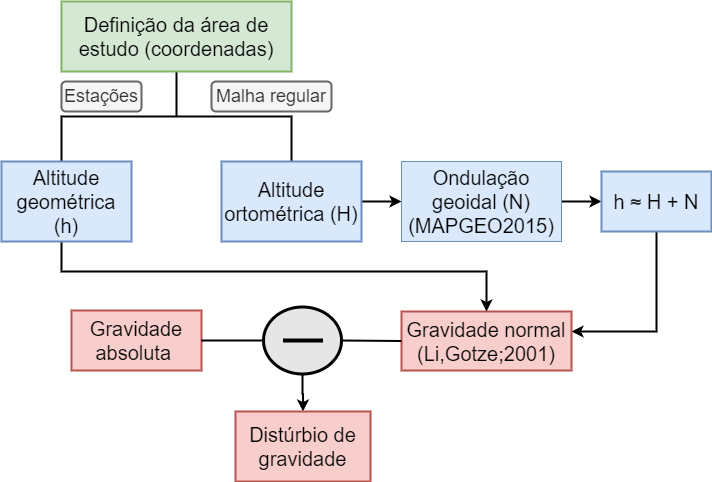
\includegraphics[scale=0.45]{figs/flux_novo.png}
	\caption{Fluxograma de trabalho adotado ao longo do desenvolvimento deste estudo.}
	\label{fig:fluxograma}
\end{figure} 

\subsection{Altitude geométrica (h)}

Como discutido no capitulo sobre fundamentação teórica, o cálculo do distúrbio de gravidade requer o conhecimento da gravidade normal. Com o efeito, a altitude geométrica é uma grandeza indispensável para que os distúrbios sejam calculados adequadamente.
 
Como descrito na seção anterior, o funcional \textit{gravity\_earth} fornece os valores de gravidade e de altitude ortométrica. Portanto, para obter as altitudes geométricas deste conjunto de pontos sobre a $SFT$ foi necessário calcular os valores de ondulação geoidal $N$. A informação referente à ondulação geoidal dos pontos de observação foi adquirida por intermédio do programa \textit{MAPGEO2015}, disponibilizado pelo site do \href{https://www.ibge.gov.br/geociencias/modelos-digitais-de-superficie/modelos-digitais-de-superficie/10855-modelo-de-ondulacao-geoidal.html?=&t=o-que-e}{IBGE}, que representa o modelo aproximado de $N$ mais recente do Brasil. Os valores de $N$, em metros, de um ponto ou conjunto
de pontos são calculados a partir das coordenadas planimétricas \cite{mapgeo2015}. De posse das altitudes ortométricas e das ondulações geoidais de cada ponto da malha regular, as altitudes geométricas puderam ser calculadas por meio da equação \ref{eq:geometric}. A Figura \ref{fig:altitude geometrica grid} mostra o mapa da malha regular referente à altitude geométrica da região da bacia do Parnaíba. É importante destacar que $H$ e $N$ foram calculados em sistemas de referências diferentes, \textit{WGS84} e \textit{SIRGAS2000}, respectivamente. No entanto, são sistemas de referência análogos e este processo não precisou ser feito para o restante dos dados, já que as medidas de campo fornecem os valores de altitude geométrica para cada estação.

\begin{figure}[H]
	\centering
	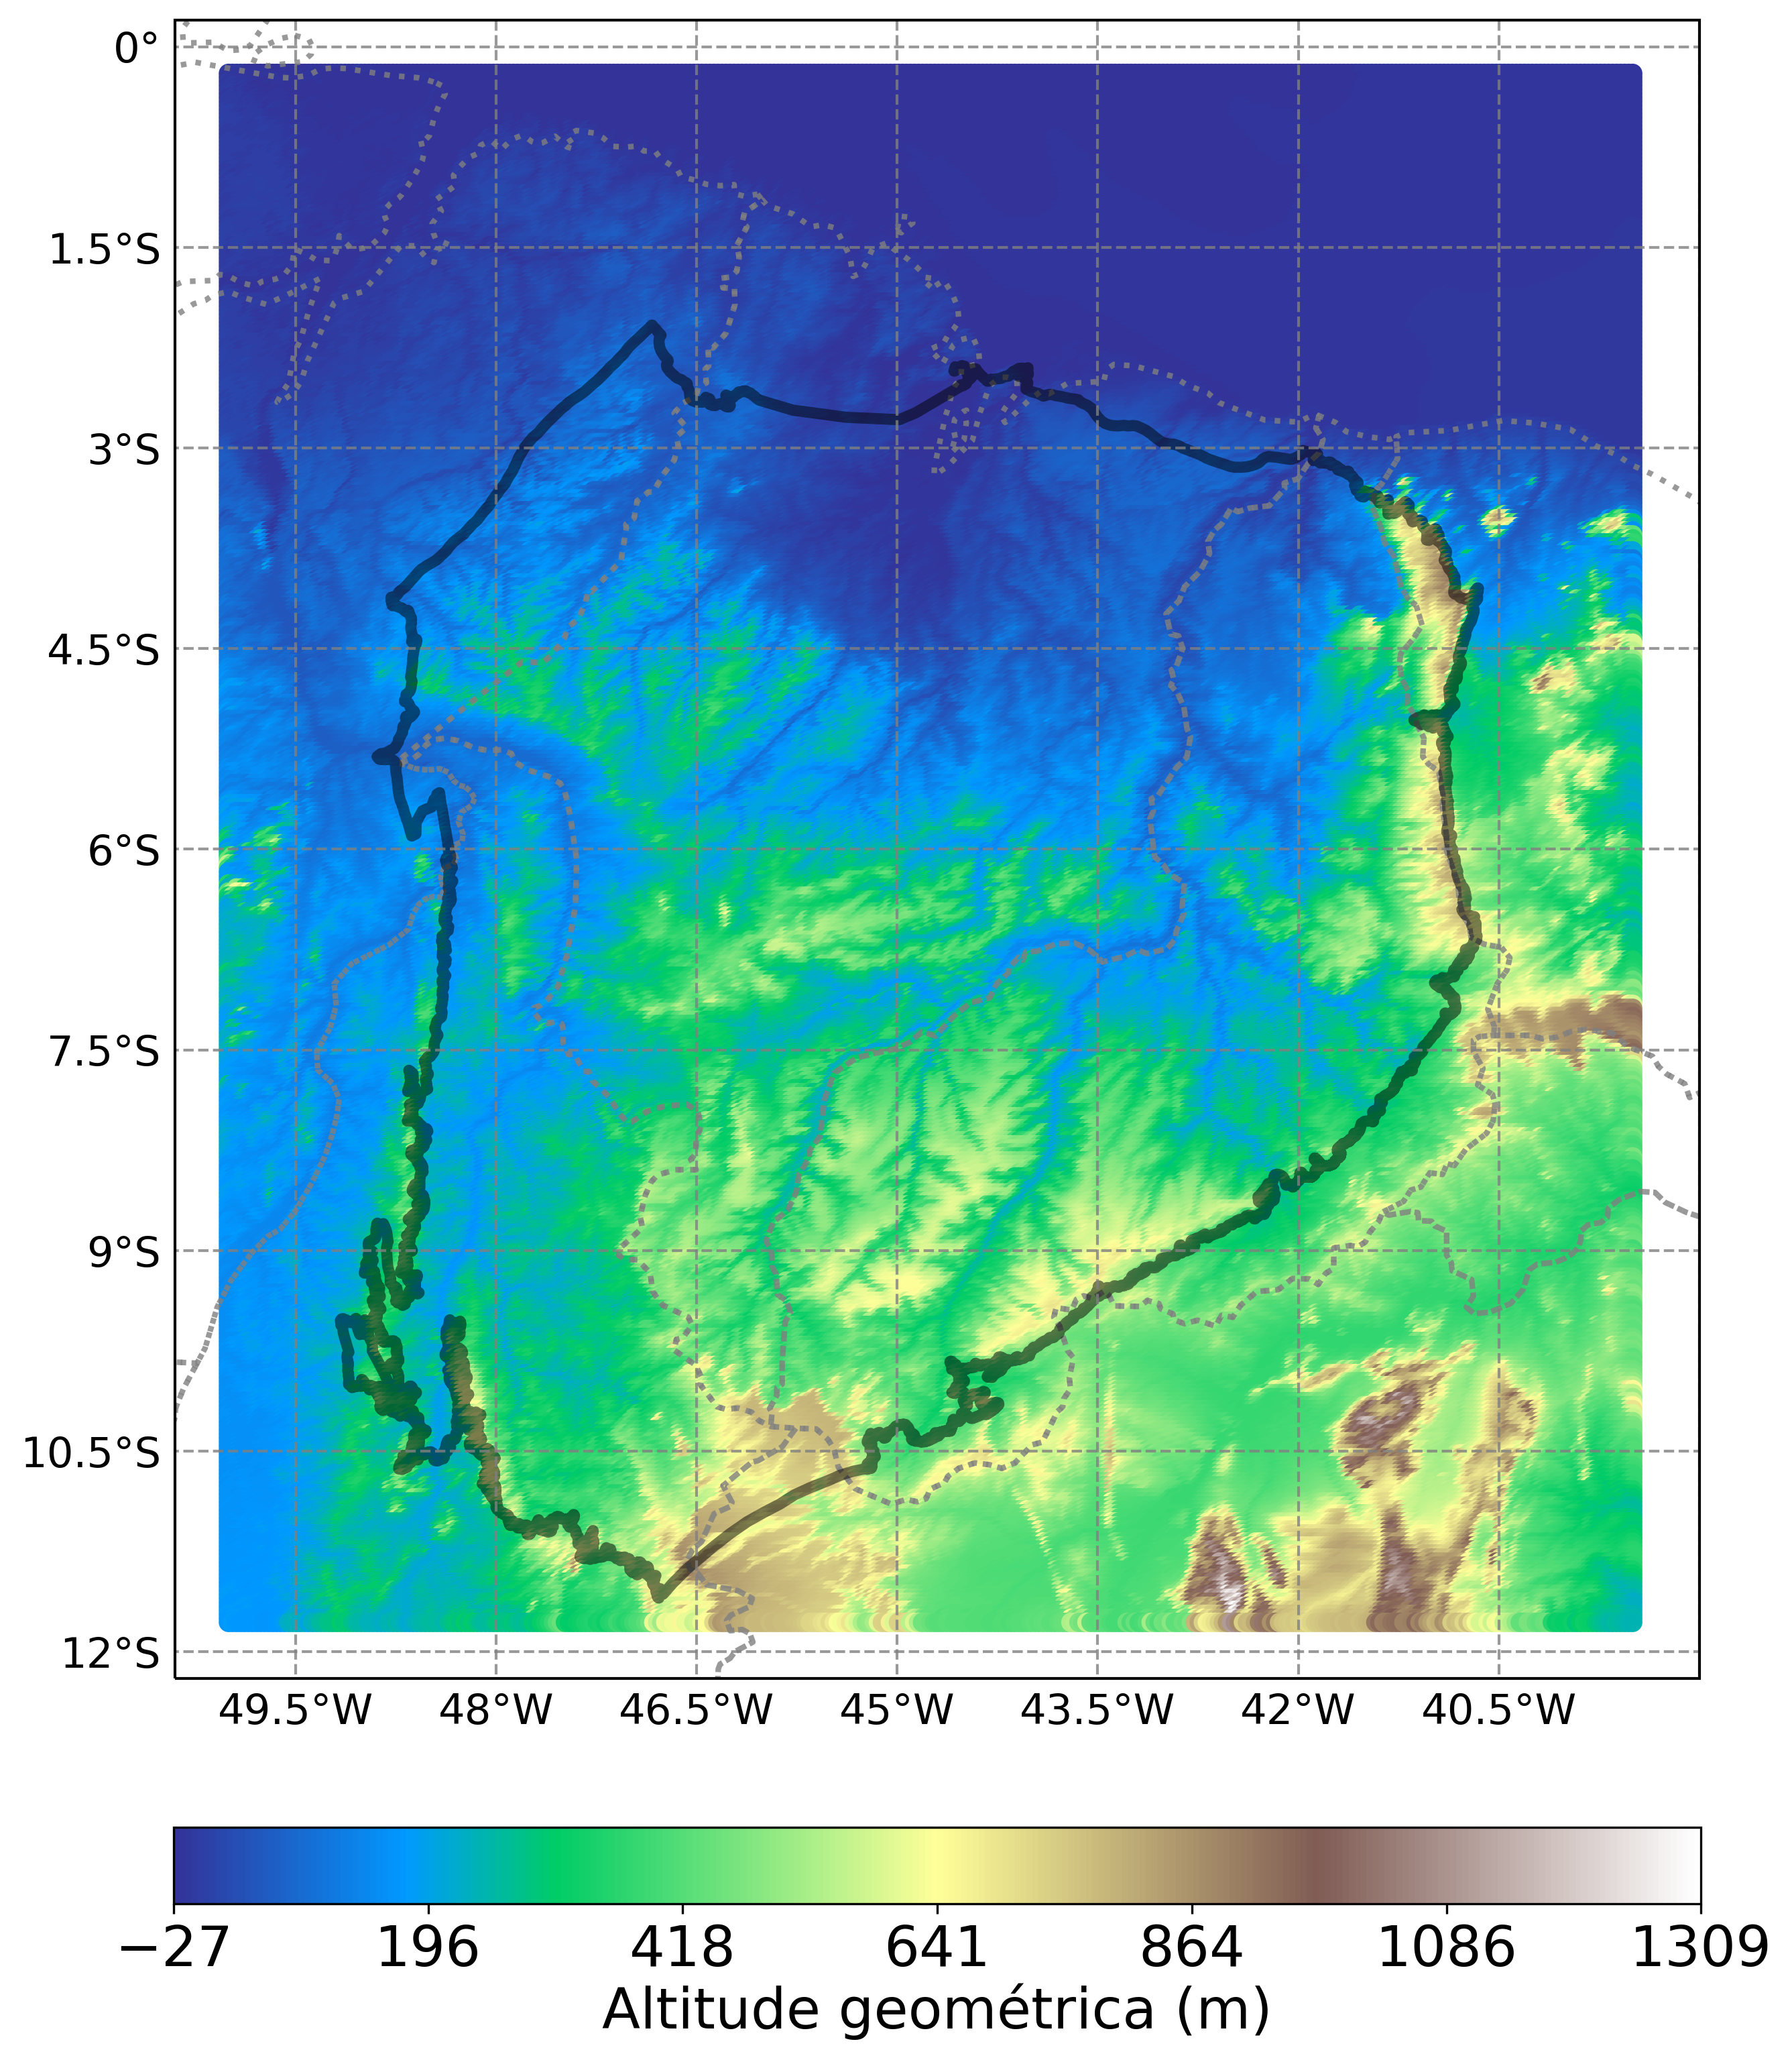
\includegraphics[scale=0.32]{figs/altitude geometrica da bacia do parnaiba.png}
	\caption{Altitude geométrica da região da bacia do Parnaíba, gerada com valores $h$ calculados a partir dos dados de $H$ do funcional \textit{gravity\_earth} e $N$ do \textit{MAPGEO2015} através da equação \ref{eq:geometric}. A região contornada em preto representa os limites da Bacia do Parnaíba e apresentou uma variação de cerca de $1309$ metros. Os contornos em cinza pontilhados representam o contorno dos estados.}	
	\label{fig:altitude geometrica grid}
\end{figure}

\subsection{Distúrbio de gravidade}
\label{subsec:delta}
Os distúrbios de gravidade foram calculados de acordo com a equação \ref{eq:disturbio}, tanto para a malha regular quanto para as estações gravimétricas terrestres. Para tal, foram utilizados os funcionais do ICGEM \textit{gravity\_earth} (para a malha) e o \textit{gravity} (para as estações). A gravidade normal, fundamental para o cálculo de $\delta g$, pode ser calculada de diversas formas. A mais comum é via fórmula internacional da gravidade, que calcula a gravidade normal sobre o elipsoide de referência \cite{somigliana}. No entanto, foi utilizada a fórmula analítica da gravidade proposta por \citeonline{li2001}, pois essa calcula a gravidade normal sobre qualquer ponto fora da Terra Normal (elipsoide). A fórmula analítica utiliza as latitudes geodésicas ($\varphi$) e as altitudes geométricas ($h$) de cada ponto analisado. Os mapas da Figura \ref{subfig:disturbio}.a, b e c mostram os dados para a malha regular. A Figura \ref{subfig:disturbio}.a representa a gravidade absoluta calculada sobre a $SFT$. É possível constatar um contraste de gravidade absoluta, principalmente na borda Leste da bacia e na região mais a Centro-Oeste, onde se nota valores mais baixos.  A Figura \ref{subfig:disturbio}.b refere-se a gravidade normal, que mostrou maior sensibilidade à $SFT$, principalmente na borda Leste, onde estão localizadas as maiores elevações da bacia. Este padrão está relacionado ao cálculo através da fórmula analítica da gravidade, que considera a altitude geométrica dos pontos. Se compararmos os mapas de gravidade absoluta e normal, nota-se um padrão homogêneo na região Nordeste no mapa da Figura \ref{subfig:disturbio}.b, que é discrepante do mapa da Figura \ref{subfig:disturbio}.a. Adicionalmente, há uma diferença significativa entre as cores de cada mapa, principalmente na porção central. Isso pode estar relacionado à questões deposicionais da bacia. Por fim, a Figura \ref{subfig:disturbio}.c mostra o distúrbio de gravidade, calculado sobre a $SFT$. É possível inferir que o depocentro da bacia está situado na porção mais ao norte, visto que, essa região apresenta um padrão de distúrbio negativo com altitude geométrica relativamente baixa. Essa conformidade nos leva a crer que a bacia têm um padrão deposicional com orientação $NE$-$SW$ \cite{tese_bacia_parnaiba}. Em sua porção Sul, em torno de ($10.5$ºS;$47$ºW), é notório que os baixos valores de distúrbio de gravidade contrastam com a topografia relativamente alta. Provavelmente, essa não conformidade pode estar associada a heterogeneidades crustais com baixos valores de contraste de densidades.
\begin{figure}[H]
	\centering
	\subfloat[Gravidade absoluta da região da bacia do Parnaíba, calculada a partir do funcional \textit{gravity\_earth}.]{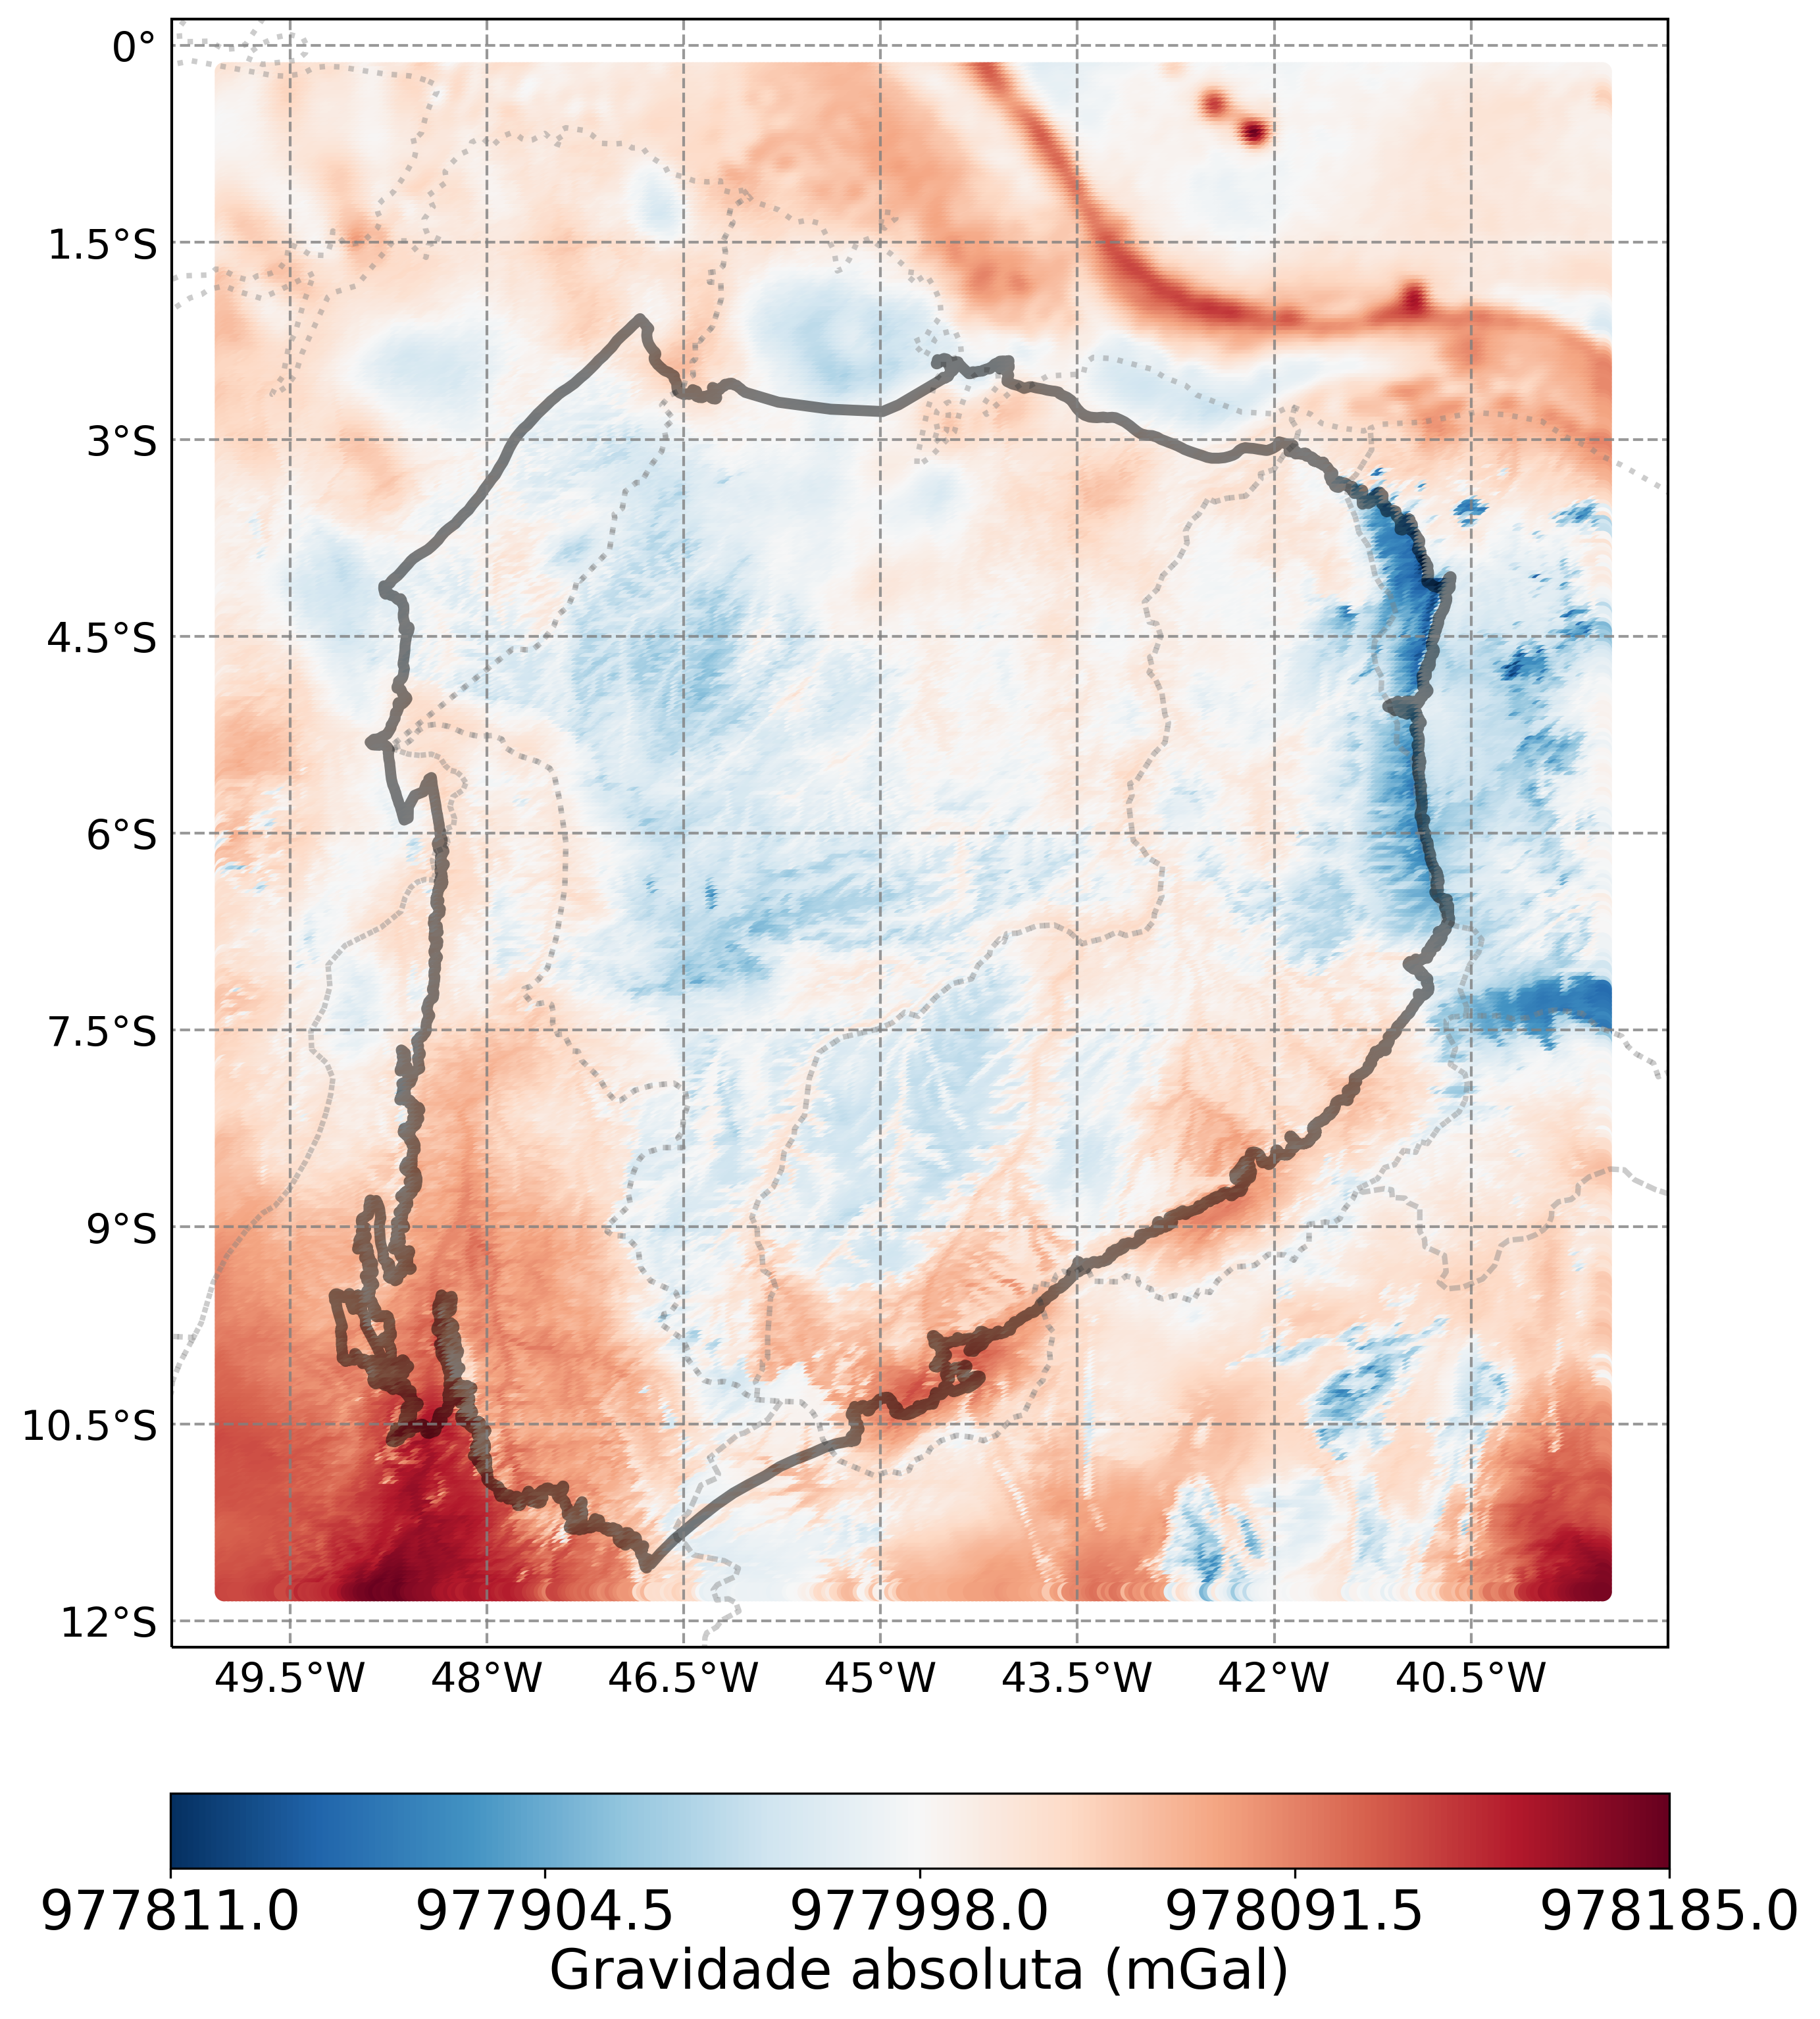
\includegraphics[scale=0.3]{figs/gravidade absoluta da bacia do parnaiba.png}} 
	\
	\subfloat[Gravidade normal da região da bacia do Parnaíba, calculada a partir da fórmula analítica da gravidade.]{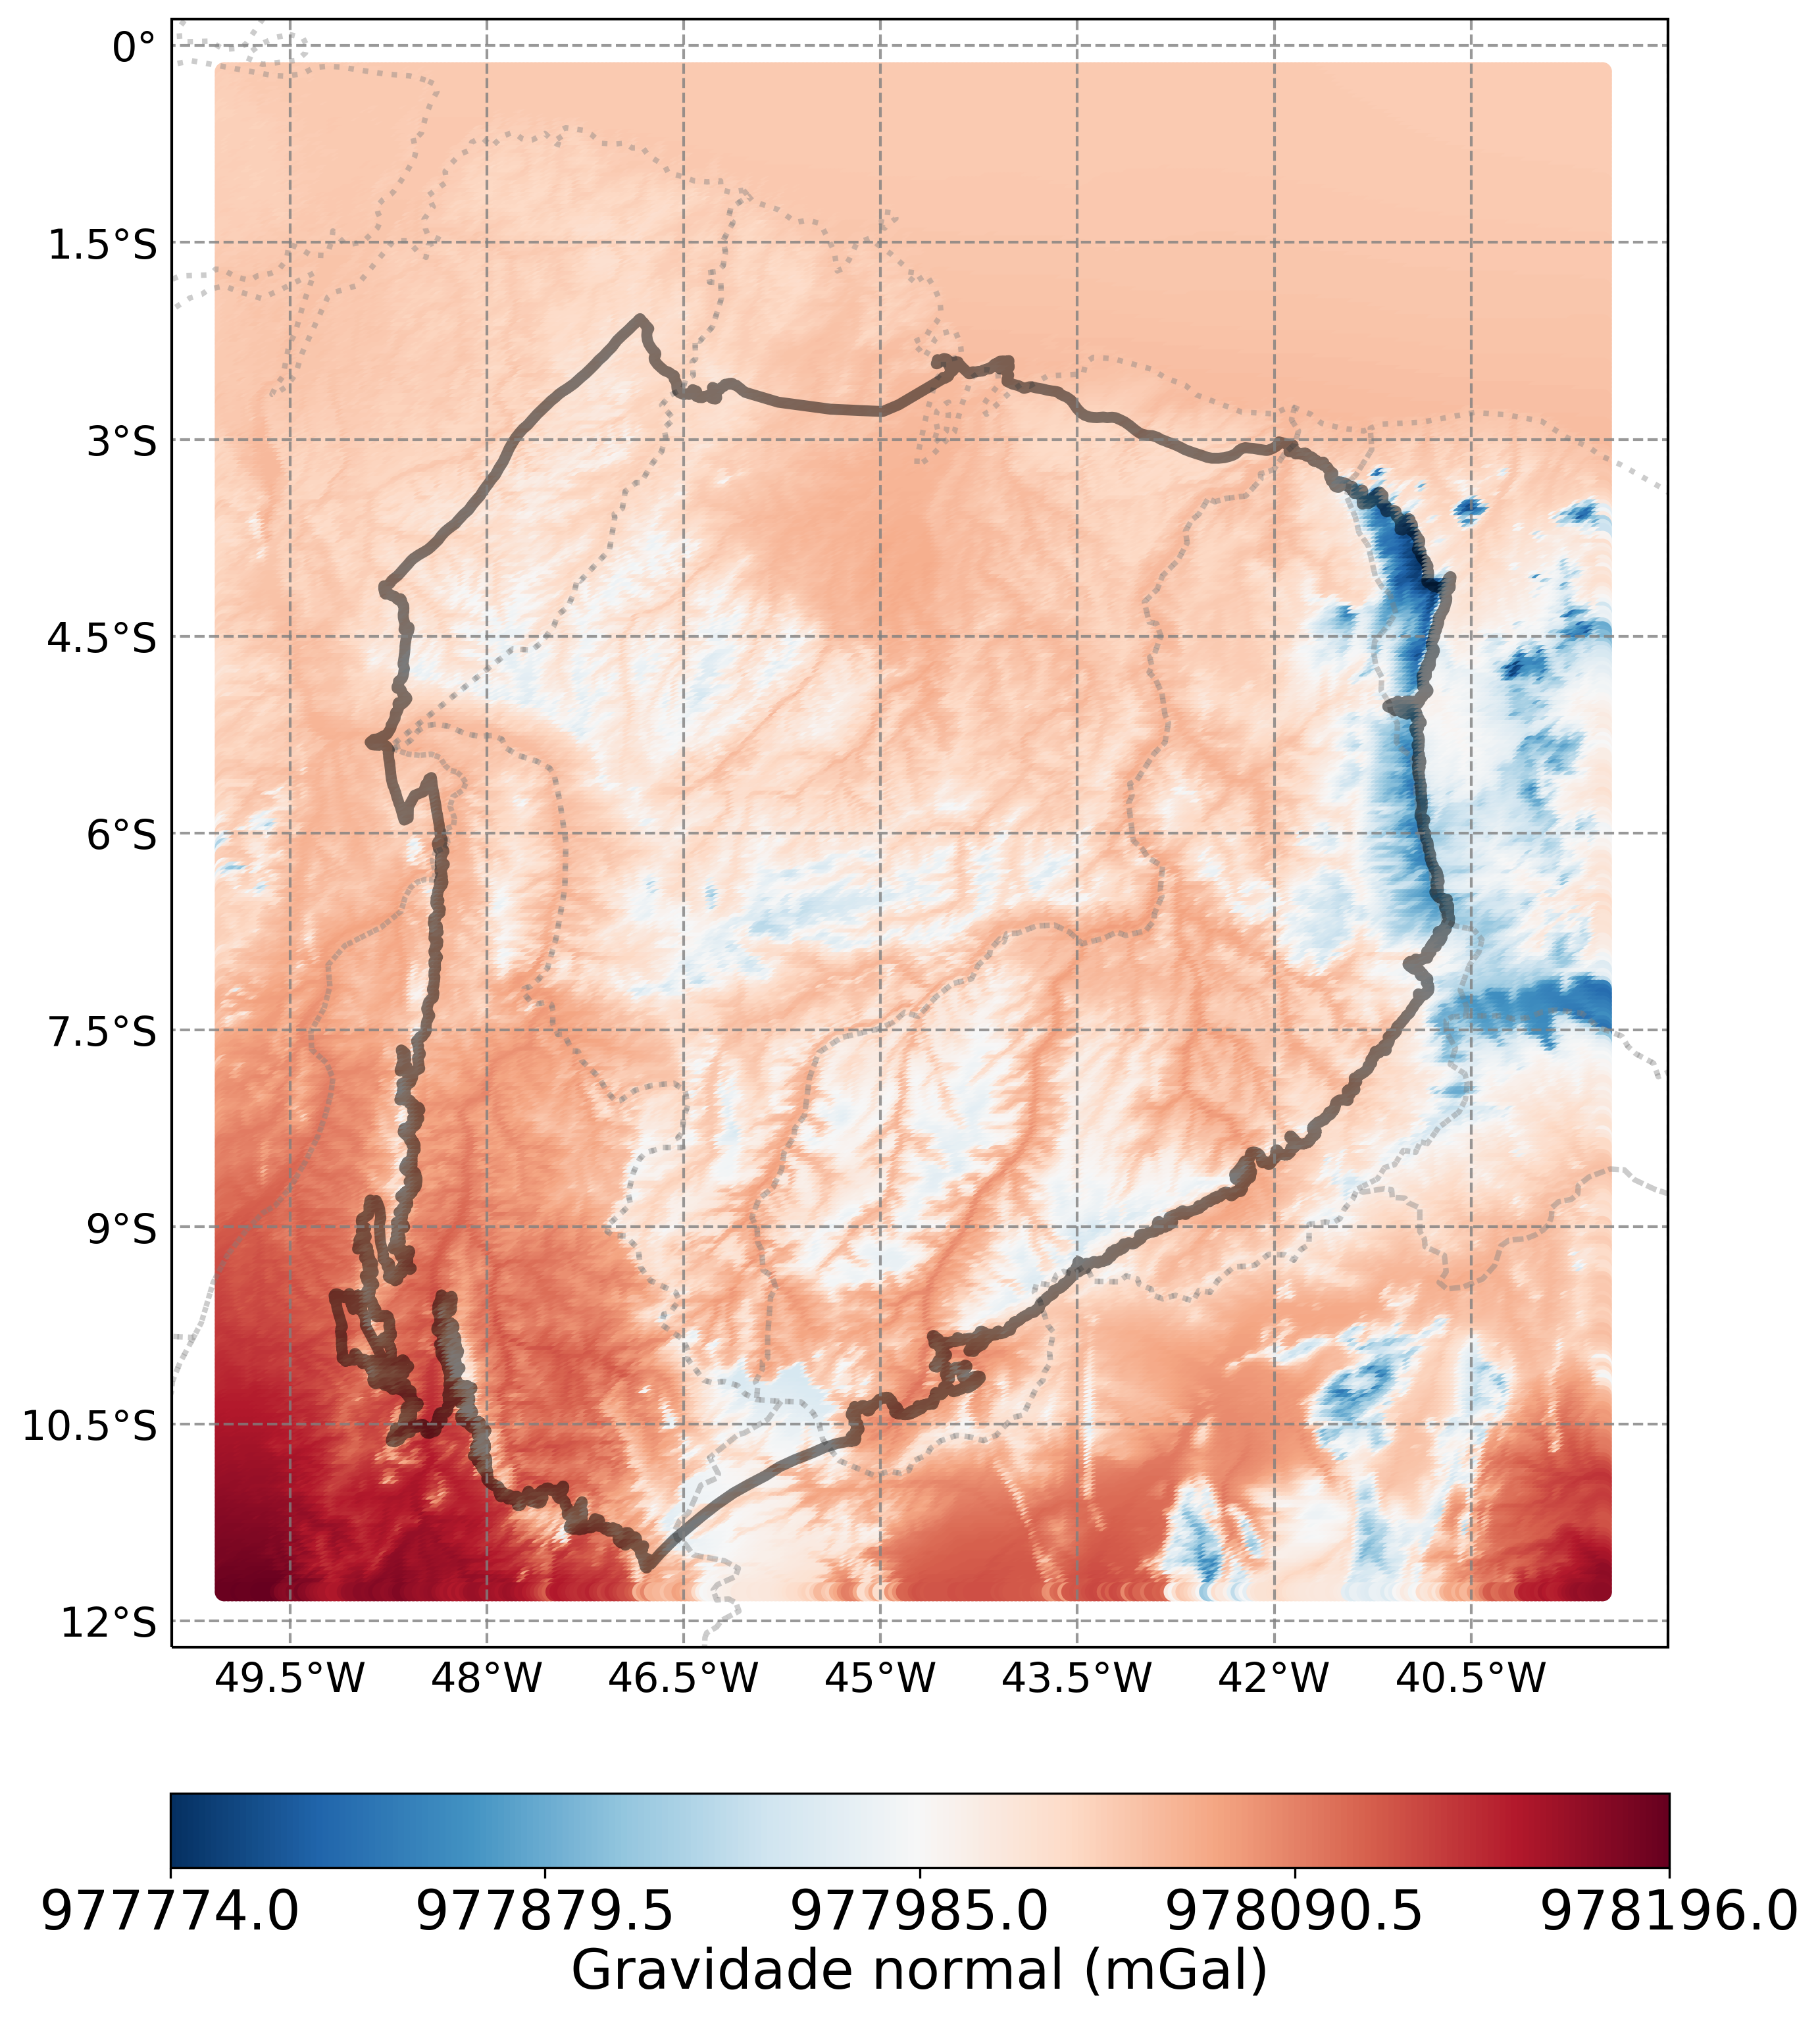
\includegraphics[scale=0.3]{figs/gravidade normal da bacia do parnaiba.png}}
	\qquad
	\subfloat[Distúrbio de gravidade da região da bacia do Parnaíba, calculado pela equação \ref{eq:disturbio}.]{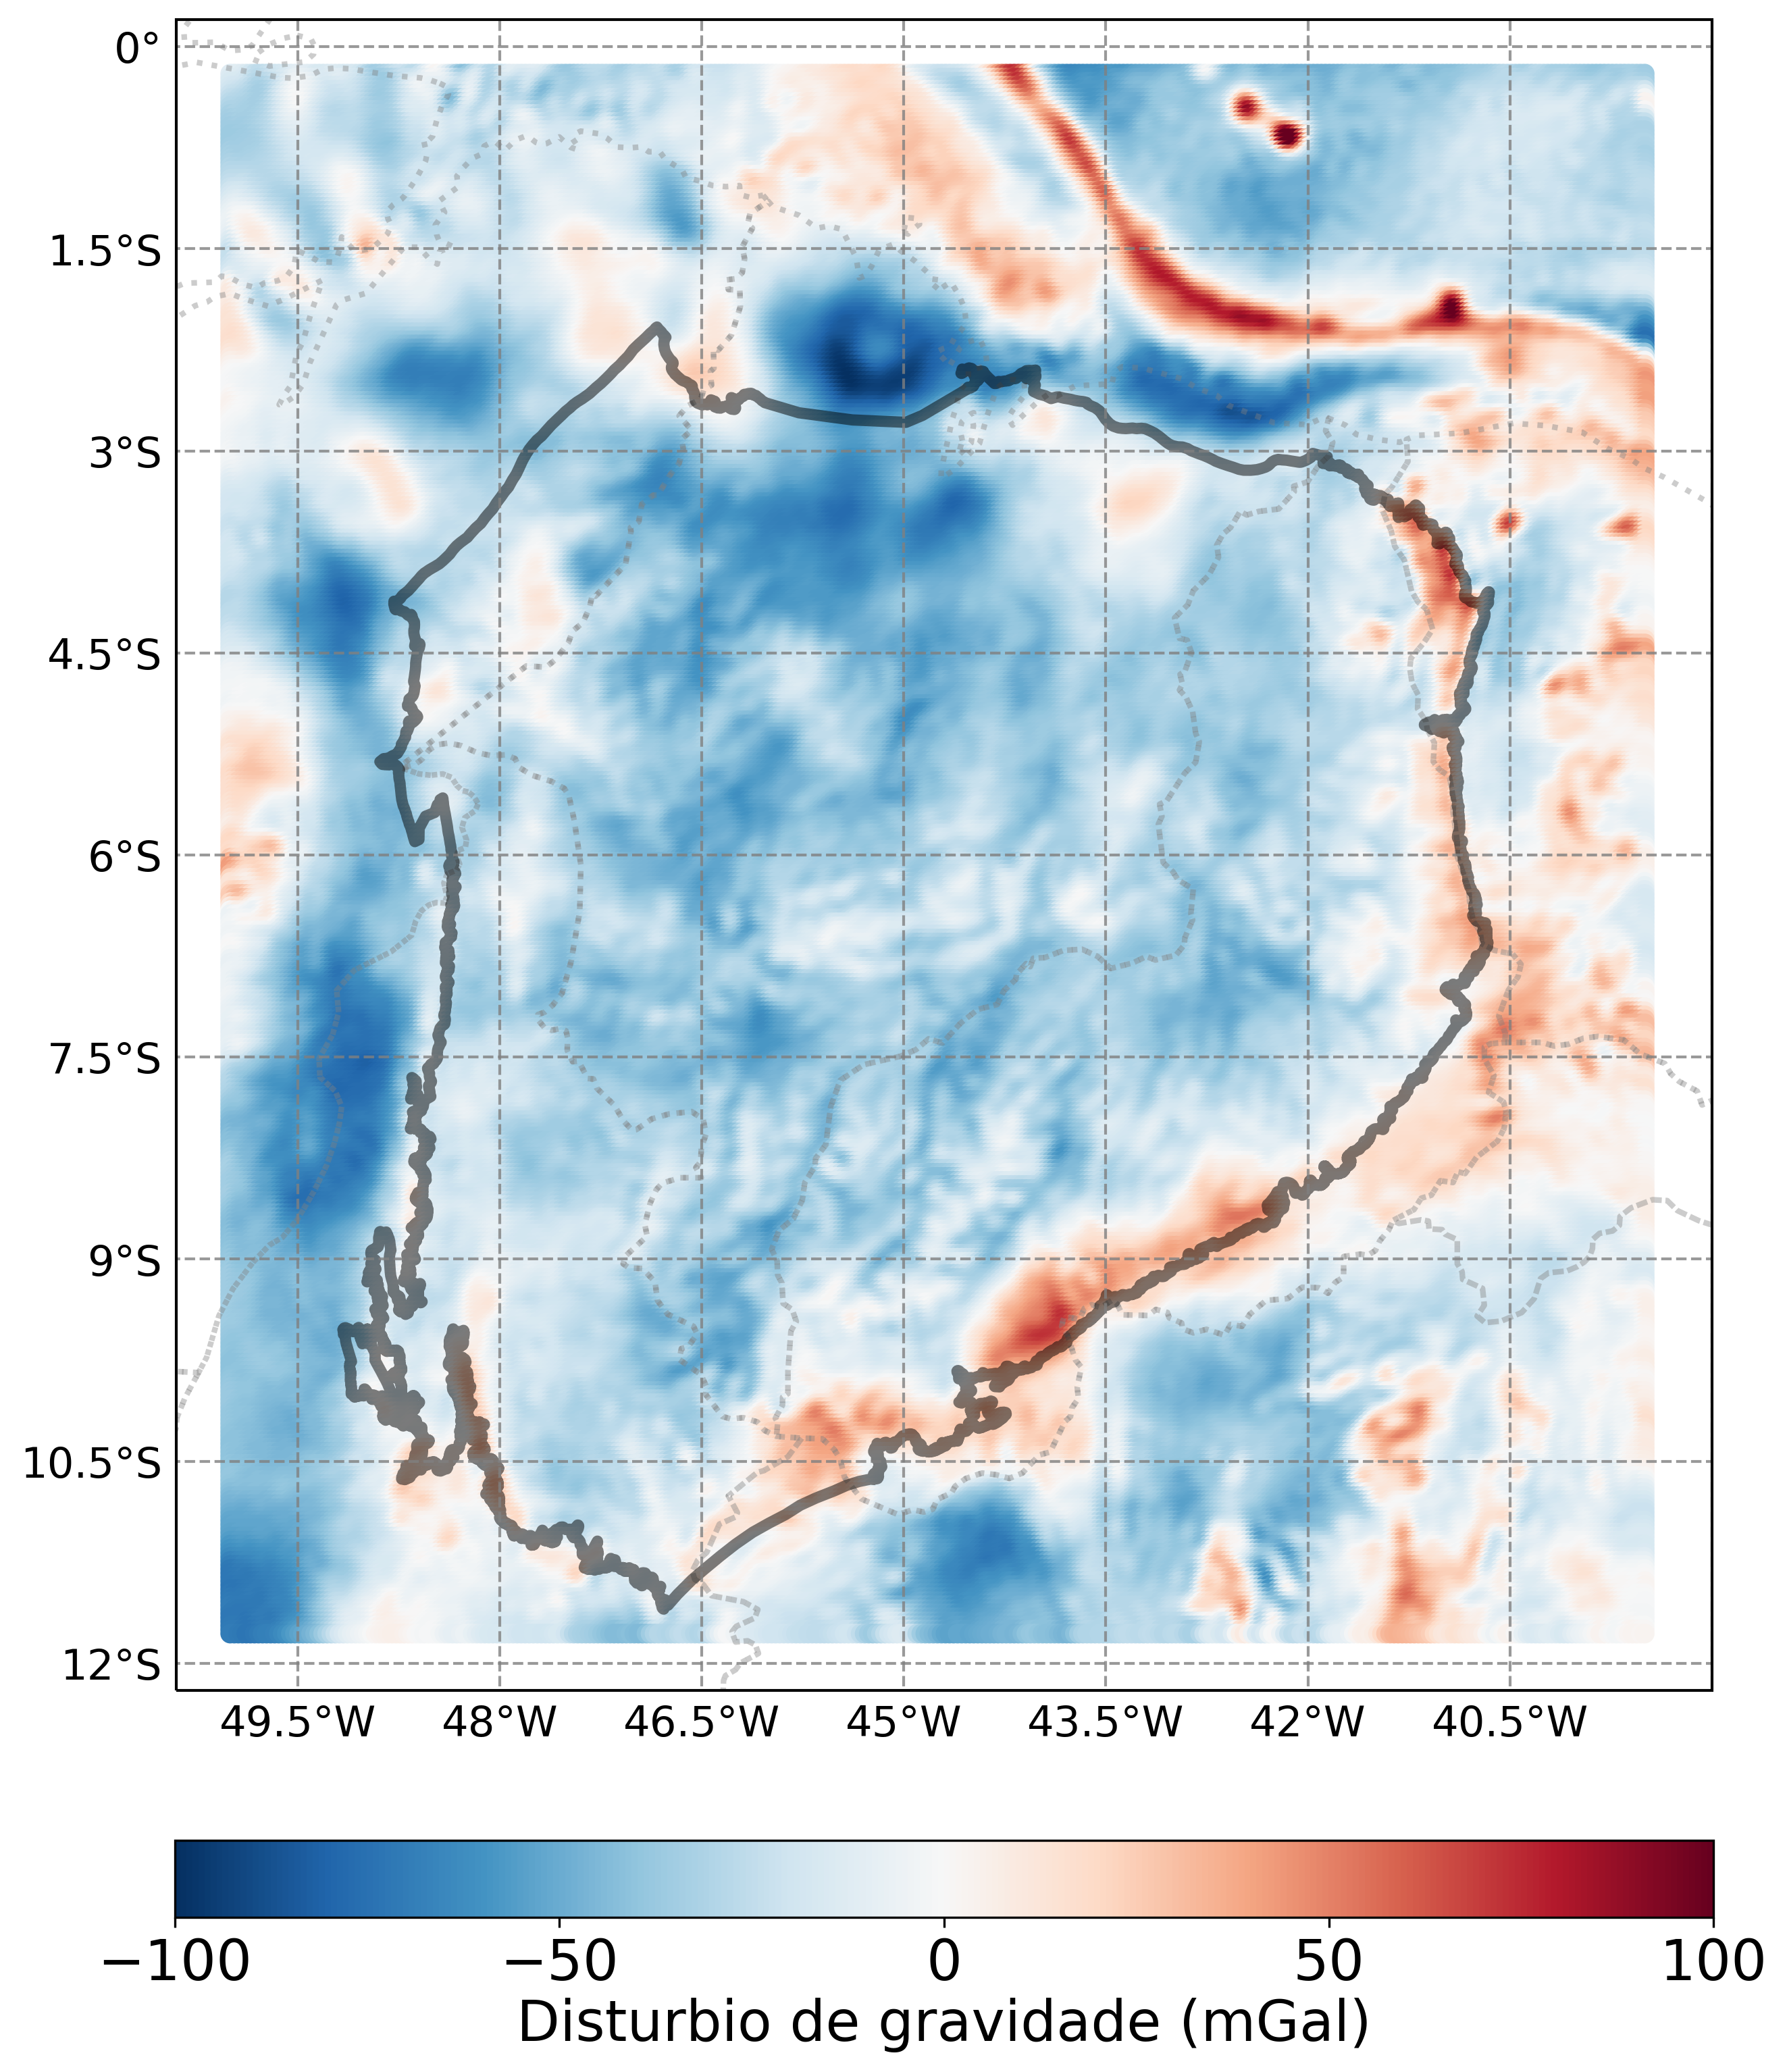
\includegraphics[scale=0.3]{figs/disturbio da bacia do parnaiba.png}}
	\caption{Malhas regulares das gravidades absoluta, normal e do distúrbio de gravidade.}  
	\label{subfig:disturbio}
\end{figure}